\documentclass{article}
\usepackage[utf8]{inputenc}

\title{Assignment 3}
\author{Rahul Krishna}
\date{1 March 2017}
\usepackage{xcolor}
\usepackage{fullpage}
\usepackage{natbib}
\usepackage{graphicx}
\usepackage{amsmath}
\usepackage{amsmath}%
\usepackage{MnSymbol}%
\usepackage{wasysym}%
\usepackage{listings}
\newcommand{\be}{\begin{equation*}\flushleft}
\newcommand{\ee}{\end{equation*}\\[0.5cm]}
\begin{document}

\maketitle
\section{PDDL Planning}
\newpage

\section{STRIPS Planning}
\begin{figure}[!h]
\centering
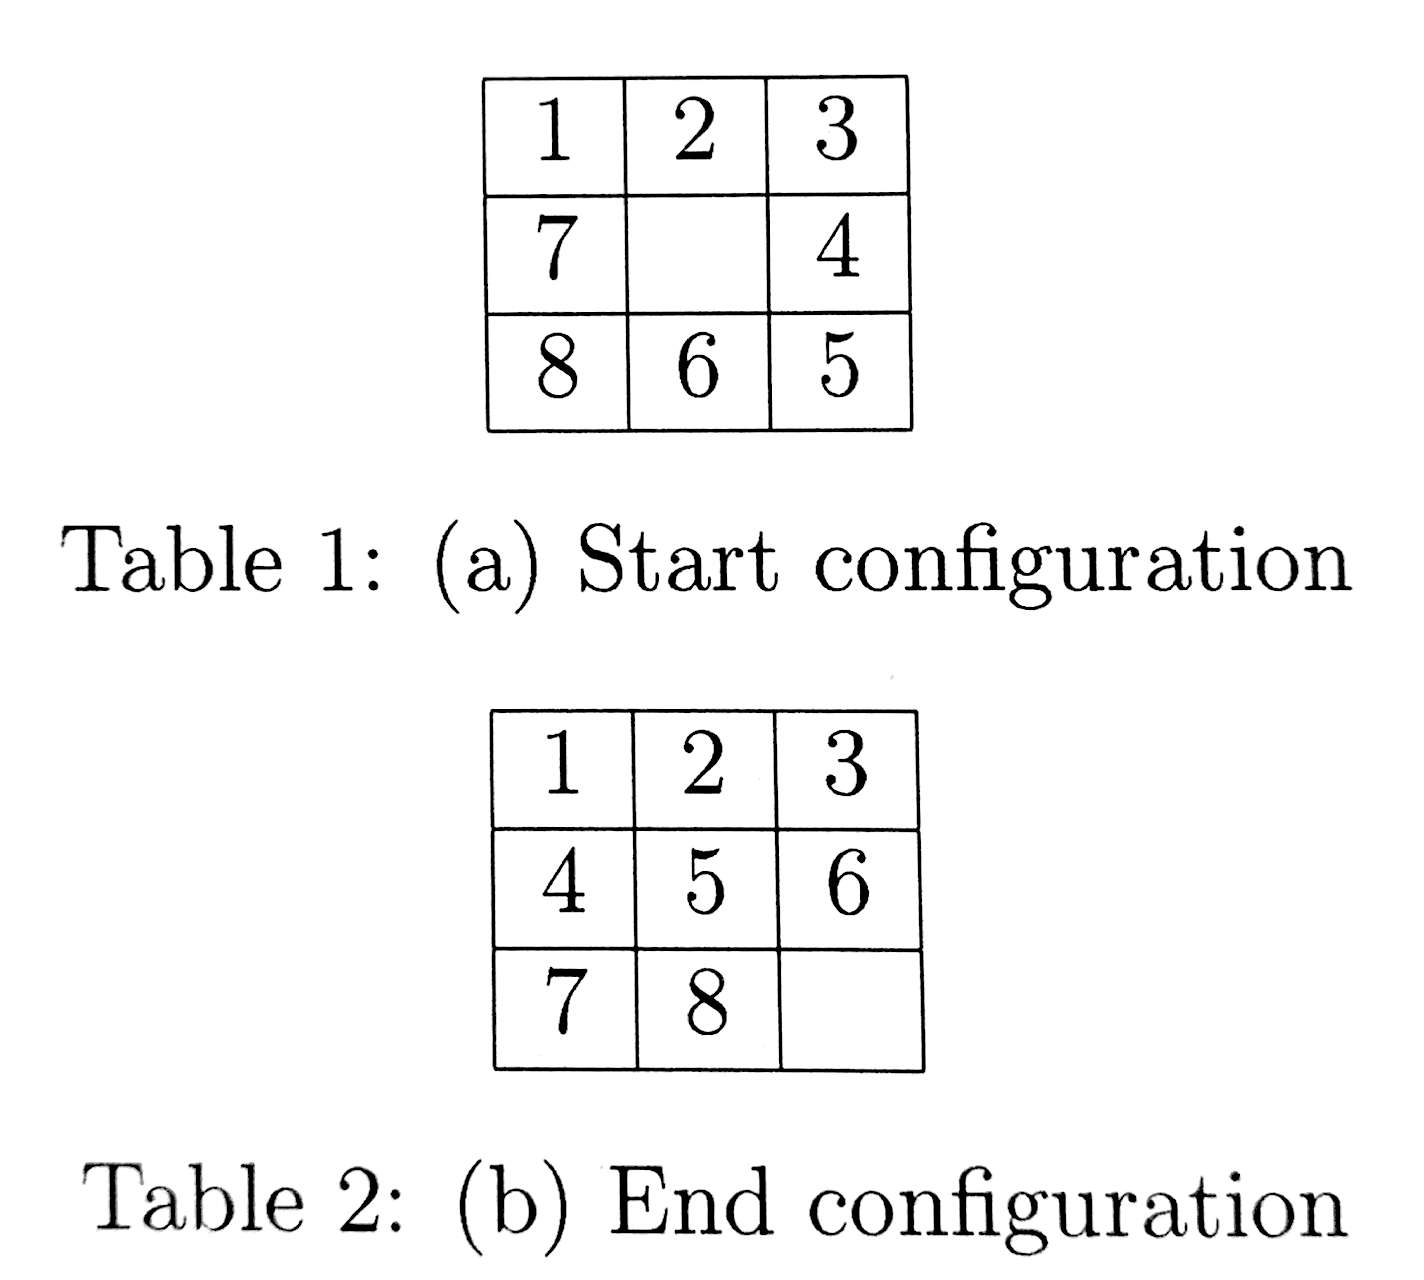
\includegraphics[width=0.33\linewidth]{assign2_q2.jpg}
\end{figure}
\subsection{Formulation}
\begin{itemize}
    \item We have 8 tiles. Let's denote them as: tile1, tile2, \ldots, tile8.
    \item We have 9 positions in a 3$\times$3 grid. Let's denote them as: pos1, pos2, \ldots, pos9.
    \item Let's use the following syntax to represent our initial and goal states:
    \begin{itemize}
        \item at(T, p): This means that a tile T is at position P.
        \item free(P): This means position P is empty.
        \item nextTo(P1, P2): This means position P1 is next (neighbour in N/E/W/S direction) to position P2.
    \end{itemize}
    \item Finally, let's define an action PUSH(T, P1, P2). PUSH must PUSH a tile T at position P1 with an entity (empty-tile) at position P2.\\ \textit{Note: We can only PUSH a tile with an empty space.}
\end{itemize}
\subsection{STRIPS}
\begin{tabular}{|p{0.95\linewidth}|}
\hline
INITIAL STATE:\\
at(tile1, pos1), at(tile2, pos2), at(tile3, pos3),at(tile7, pos4), free(pos5), at(tile4, pos6), at(tile8, pos7), at(tile6, pos8), at(tile5, pos9)\\[3pt]
nextTo(pos1, pos2), nextTo(pos2, pos1), nextTo(pos2, pos3), nextTo(pos3, pos2), nextTo(pos3, pos4), nextTo(pos4, pos3), nextTo(pos4, pos5), nextTo(pos5, pos4), nextTo(pos5, pos6), nextTo(pos6, pos5), nextTo(pos6, pos7), nextTo(pos7, pos6), nextTo(pos7, pos8), nextTo(pos8, pos7), nextTo(pos8, pos9), nextTo(pos9, pos8), nextTo(pos1, pos4), nextTo(pos4, pos1), nextTo(pos2, pos5), nextTo(pos5, pos2), nextTo(pos3, pos6), nextTo(pos6, pos3), nextTo(pos4, pos7), nextTo(pos7, pos4), nextTo(pos5, pos8), nextTo(pos8, pos5), nextTo(pos6, pos9), nextTo(pos9, pos6)
\\\hline
GOAL STATE:\\
at(tile1, pos1), at(tile2, pos2), at(tile3, pos3),at(tile4, pos4), at(tile5, pos5), at(tile6, pos6), at(tile7, pos7), at(tile9, pos8), free(pos9)\\\hline
ACTIONS:\\
\hspace{8pt}PUSH(T,P1,P2):\\
\hspace{16pt}PRECONDITIONS: $\text{at(T,P1)}\land \text{nextTo(P1,P2)}\land \text{free(P2)}$\\
\hspace{16pt}EFFECTS: $\text{at(T,P2)}\land \text{!free(P2)}\land \text{!at(T,P1)}\land \text{free(P1)}$\\\hline
\end{tabular}
\end{document}
